\documentclass[9pt,oneside]{amsart}

%\usepackage{tweaklist}
\usepackage{cancel}
\usepackage{xspace}
\usepackage[utf8]{inputenc}
\usepackage{graphicx}
\usepackage{multicol}
\usepackage{subfig}
\usepackage{amsmath}
\usepackage{amssymb}
\usepackage[a4paper,width=170mm,top=18mm,bottom=22mm,includeheadfoot]{geometry}
\usepackage{booktabs}
\usepackage{array}
\usepackage{verbatim}
\usepackage{caption}
% \usepackage{natbib}

\usepackage{float}
\usepackage{pdflscape}
\usepackage{mathtools}
\usepackage[usenames,dvipsnames]{xcolor}
\usepackage{afterpage}
\usepackage{tikz}
\usepackage[bookmarks=true, unicode=true, pdftitle={Ethereum Yellow Paper: a formal specification of Ethereum, a programmable blockchain}, pdfauthor={Dr. Gavin Wood},pdfkeywords={Ethereum, Yellow Paper, blockchain, virtual machine, cryptography, decentralised, singleton, transaction, generalised},pdfborder={0 0 0.5 [1 3]}]{hyperref}
%,pagebackref=true

\usepackage{tabu} %requires array.

%This should be the last package before \input{Version.tex}
\PassOptionsToPackage{hyphens}{url}\usepackage{hyperref}
% "hyperref loads the url package internally. Use \PassOptionsToPackage{hyphens}{url}\usepackage{hyperref} to pass the option to the url package when it is loaded by hyperref. This avoids any package option clashes." Source: <https://tex.stackexchange.com/questions/3033/forcing-linebreaks-in-url/3034#comment44478_3034>.
% Note also this: "If the \PassOptionsToPackage{hyphens}{url} approach does not work, maybe it's "because you're trying to load the url package with a specific option, but it's being loaded by one of your packages before that with a different set of options. Try loading the url package earlier than the package that requires it. If it's loaded by the document class, try using \RequirePackage[hyphens]{url} before the document class." Source: <https://tex.stackexchange.com/questions/3033/forcing-linebreaks-in-url/3034#comment555944_3034>.
% For more information on using the hyperref package, refer to e.g. https://en.wikibooks.org/w/index.php?title=LaTeX/Hyperlinks&stable=0#Hyperlink_and_Hypertarget.

\makeatletter
 \newcommand{\linkdest}[1]{\Hy@raisedlink{\hypertarget{#1}{}}}
\makeatother
\usepackage{seqsplit}

% For formatting
%\usepackage{underscore}
%\usepackage{lipsum} % to generate filler text for testing of document rendering
\usepackage[english]{babel}
\usepackage[autostyle]{csquotes}
\MakeOuterQuote{"}

\usepackage[final]{microtype} % https://tex.stackexchange.com/questions/75140/is-it-possible-to-make-latex-mark-overfull-boxes-in-the-output#comment382776_75142


% \input{Version.tex}
% Default rendering options
\definecolor{pagecolor}{rgb}{1,0.98,0.9}
\def\YellowPaperVersionNumber{unknown revision}
\IfFileExists{Options.tex}{\input{Options.tex}}

\newcommand{\hcancel}[1]{%
    \tikz[baseline=(tocancel.base)]{
        \node[inner sep=0pt,outer sep=0pt] (tocancel) {#1};
        \draw[black] (tocancel.south west) -- (tocancel.north east);
    }%
}%


\DeclarePairedDelimiter{\ceil}{\lceil}{\rceil}
\newcommand*\eg{e.g.\@\xspace}
\newcommand*\Eg{e.g.\@\xspace}
\newcommand*\ie{i.e.\@\xspace}
%\renewcommand{\itemhook}{\setlength{\topsep}{0pt}  \setlength{\itemsep}{0pt}\setlength{\leftmargin}{15pt}}


\title{ETH-Paid Internet Access\\ {\smaller \textbf{Proyecto final de máster (versi\'on texto en Español)}}}
\author{
    A. Egio, L. González, A. Pardo, T. Romero\\
    UPC School, Carrer de Badajoz 73, 08005 Barcelona - Catalunya\\
    E-mail: [alfonsoea, lluisgv2, albertopm5, joserc25]
}

\begin{document}

\pagecolor{pagecolor}


\begin{abstract}
  This document shows a new solution to get Internet acces to users
  using Wifi networks. The innovation is about to add a time
  per use payment gateway
  using the ethereum ETH crytocurrency and
  tokens (new Ethereum's cryptoactives).
  %% Este documento presenta una soluci\'on novedosa para habilitar el acceso a Internet a usuarios mediante redes Wi-Fi. La innovaci\'on consiste en añadir
  %% una pasarela de pago por tiempo de uso a través
  %% de criptomonedas ETH de Ethereum y tokens
  %% (nuevos criptoactivos de Ethereum).
  %% Se describe la construcci\'on de un
  %% prototipo basado en hardware libre (Raspberry Pi) para llevar a cabo la prueba de concepto. Paralelamente, se estudia la viabilidad de negocio en torno a ello. Por ejemplo, orientado a ciudades/ayuntamientos.
\end{abstract}

\maketitle

\tableofcontents


\setlength{\columnsep}{20pt}
\begin{multicols}{2}
\section{Introducci\'on}\label{sec:introduction}
\paragraph
\noindent
Internet access nowadays has become a key factor
and a must for information society. Currently and depending
on geographical location, internet access
can be provided by local area networks [Stallings 04].
Due to its characteristics wireless networks
are ideal for movility and ease of configuration
and maintenance. WiFi technology has become
a de-facto standard.


Por otro lado, la irrupción en los últimos
años de la tecnología Blockchain
ha traído consigo un nuevo paradigma
en el desarrollo de aplicaciones
descentralizadas (en adelante, \DH App).
Las criptomonedas (tales como Bitcoin
[Nakamoto 08], ETH de Ethereum,
XRP de Ripple, etc.)
son una de las primeras aplicaciones. Éstas suponen
una nueva forma de pago e intercambio de dinero más eficiente a la tradicional (emitida por bancos centrales y de forma centralizada).

%\subsection{Background} \label{ch:backg}
\subsection{Base tecnológica} \label{ch:backg}

Blockchain es una lista de registros en continuo crecimiento llamados bloques. Están enlazados y asegurados mediante criptografía. Adopta el protocolo P2P (\textit{peer-to-peer}) que puede tolerar un único punto de fallo. El mecanismo de consenso asegura un orden común e inequívoco de las transacciones y bloques, y garantiza la integridad y consistencia de la cadena de bloques a través de nodos distribuidos geográficamente. Por su diseño, la cadena de bloques tiene características tales como: descentralización, integridad y auditabilidad. La cadena de bloques puede servir como un nuevo tipo de conector de software, que debería considerarse como una posible alternativa descentralizada al almacenamiento de datos compartido centralizado existente.

Además, en función de los diferentes niveles de permiso de acceso, las cadenas de bloques pueden dividirse en dos tipos: 1) pública (tales como Bitcoin y Ethereum); y 2) privada (tal y como Hyperledger). Blockchain sirve como plataforma para los contratos inteligentes (en adelante, \textit{smart contracts}). Por ejemplo, programados en lenguaje Solidity de Ethereum, se alojen y ejecuten. Blockchain es un concepto de tecnología de libro mayor distribuido DLT (\textit{distributed ledger technology}). Se puede integrar en múltiples áreas de negocio.

\subsection{Trabajos similares encontrados} \label{ch:similar}
En la literatura se recogen trabajos similares realizados para la compartición de la banda ancha del espectro radioeléctrico en redes Wi-Fi.

Algunos son éstos:
\subsubsection{Fon} \label{ch:fon}
Surge en el año 2005 con el objetivo de crear una comunidad Wi-Fi global, que permita a sus usuarios la conexión gratuita a los puntos de acceso de otros usuarios. Del mismo modo, brinda acceso de pago a terceros mediante un sistema en el que las ganancias se reparten entre Fon y el
usuario que presta su conexión. El sistema facilita medios de pago electrónicos (no Blockchain) a estos no usuarios. Han desarrollado y puesto a la venta sus propios routers a los que llama Fonera (véase figura 1).
\begin{center}
%\begin{figure}[h]
%  \centering
  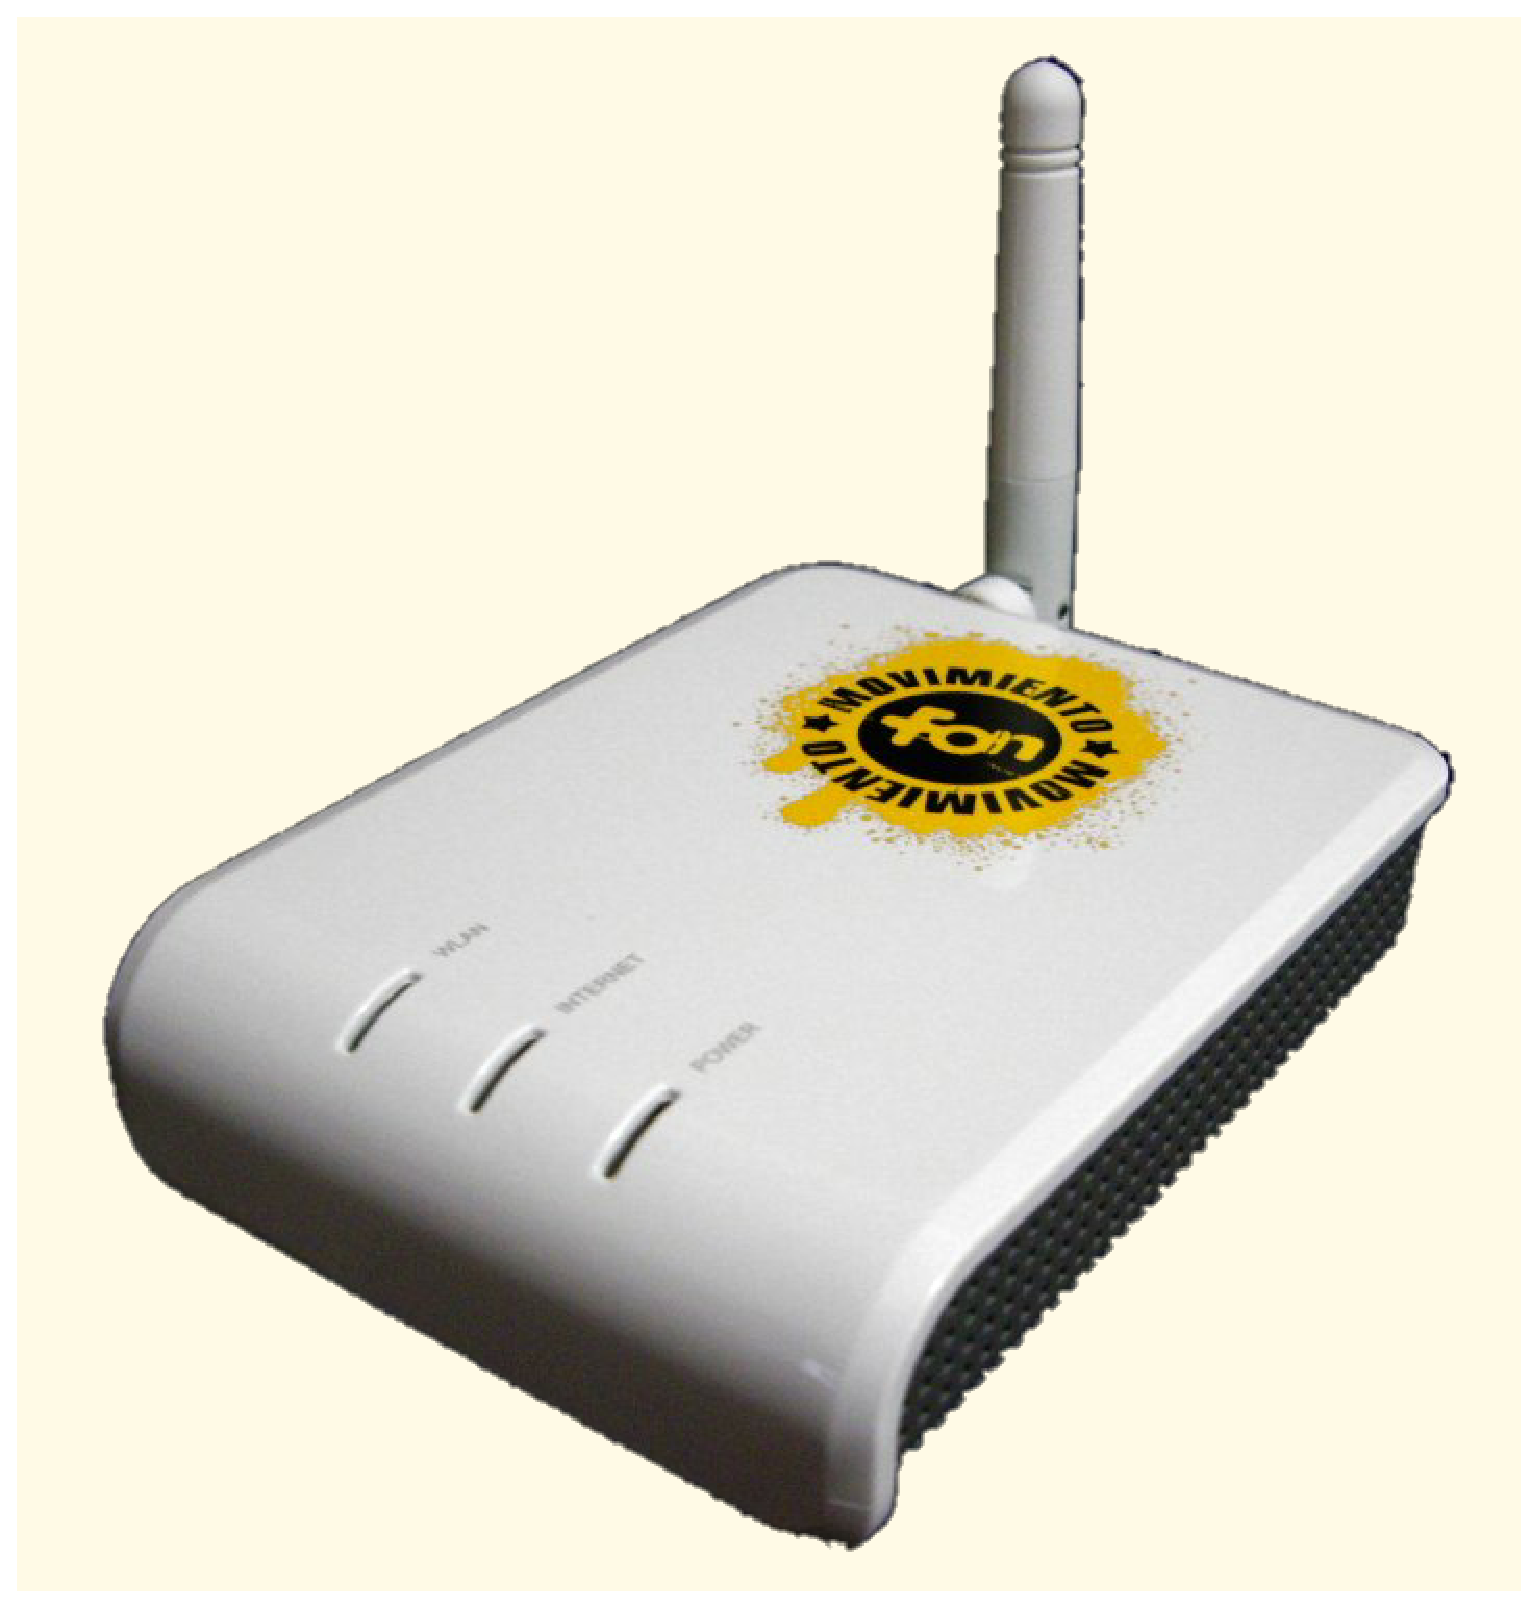
\includegraphics[keepaspectratio, width=0.2\textwidth]{images/lafonera-sourcewikipedia.eps}
%  \caption{Figura 1. La Fonera}
%\end{figure}
\\
Figura 1. La Fonera. Fuente: Wikipedia.
\\
\end{center}
\subsubsection{Hotspot me de Hackathon ETH Berlín Zwei} \label{ch:ethberlinzwei}
En el año 2019 durante esta hackathon de los días 23-25 de Agosto resultó ganadora una aplicación que permite a un local proporcionar su punto de acceso de forma anónima mediante DAI (una criptomoneda) [ETHBerlínZwei 19].
\section{Solución propuesta}\label{sec:solution}
La solución basada en \DH App propuesta se describe a continuación:
\subsection{Diseño} \label{ch:design}
(Por completar)
\subsubsection{Roles} \label{ch:roles}
(Por completar)
\\
\\
\textit{ETH-Paid hotspot provider} (E-Php).
\\
\\
\textit{Hotspot handler} (hh).
\\
\\
\textit{Upstream Internet Service Provider} (U-ISP).
\\
\\
Usuario.
\subsubsection{Arquitectura} \label{ch:architecture}
(Por completar)
\\
\\
Gestión del stake.
\subsection{Implementación} \label{ch:implementation}
El estudio del equipamiento a utilizar es importante en cualquier proyecto. En esta sección se hará una breve introducción de los principales componentes con los que se ha trabajado. También se indicará cómo se debe preparar la prueba de concepto (en adelante, PoC).
\subsubsection{Front-end} \label{ch:front-end}
(Por completar)
\subsubsection{Back-end} \label{ch:back-end}
(Por completar)
\\
\\
Raspberry Pi.
\\
\\
Se ha utilizado la Raspberry Pi 3 Modelo B (véase figura 2). Un ordenador de placa reducida SBC (\textit{single board computer}).
\begin{center}
%\begin{figure}[h]
%  \centering
  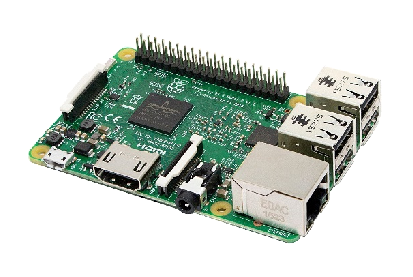
\includegraphics[keepaspectratio, width=0.2\textwidth]{images/rpi3modelb-sourceamazon.eps}
%  \caption{Figura 2. Raspberry Pi 3 Modelo B. Fuente: [Raspberry 18]}
%\end{figure}
\\
Figura 2. Raspberry Pi 3 Modelo B. Fuente: [RaspberryPi 19]
\\
\end{center}
Un resumen de sus especificaciones se da a continuación (véase tabla 1):
\begin{center}
%\begin{tabular} to 0.5\textwidth { | X[l] | X[r] | }
\begin{tabular}{ | m{0.125\textwidth} | m{0.3125\textwidth} | }
 \hline
 Especificaciones & Raspberry Pi 3 Modelo B \\
 \hline
 Procesador & Broadcom BCM2837, Cortex-A53 (ARMv8) 64-bit SoC @ 1,2 GHz \\
\hline
 RAM & 1 GB \\
\hline
 Conectividad & Wi-Fi 802.11 b/g/n (2,4 GHz) Bluetooth 4.1 Puerto Ethernet de hasta 100 Mbps \\
\hline
 Puertos & HDMI completo, 4 USB 2.0, MicroSD, CSI camera, DSI display \\
\hline
 Memoria & MicroSD \\
\hline
\end{tabular}
\newline
\end{center}
Tabla 1. Especificaciones de Raspberry Pi 3 Modelo B
%\newline
\\
\\
Aunque no se indica expresamente si es hardware libre (\textit{open hardware}) o con derechos de marca, en su página Web oficial explican que disponen de contratos de distribución y venta con dos empresas. Pero al mismo tiempo, cualquiera puede convertirse en revendedor o redistribuidor de las tarjetas Raspberry Pi [RaspberryPiBuy 19].
\\
\\
Smart contracts.
\\
\\
La parte smart contract consiste en un smart contract para pago con ETH y otro smart contract para pago con tokens.
\begin{itemize}
 \item Smart contract ETH
 \item Smart contract token
 \newline
\end{itemize}
(Por completar)
\section{Pruebas}\label{sec:proofs}
Para validar la PoC, se ha definido una batería de tests. Por ejemplo, dado que los smart contract normalmente manejan dinero, es esencial asegurarse de que su número de fallos y vulnerabilidades sea bajo [Hegedus 18]. Para ayudar a los desarrolladores y hacer más madura la tecnología, necesitamos herramientas de análisis [ConsenSys 19].
\subsection{Tests} \label{ch:tests}
(Por completar)
\section{Despliegue}\label{sec:deploy}
Docker es una herramienta que permite desplegar aplicaciones dentro de contenedores de software. Esto puede ser útil para la Raspberry Pi porque permite a los usuarios ejecutar aplicaciones con muy poca sobrecarga, siempre y cuando la aplicación esté empaquetada dentro de una imagen Docker. Simplemente instalamos Docker y ejecutamos el contenedor sobre Raspbian/ARM. Éste despliega el proyecto realizado.

La secuencia de comandos a ejecutar es:
\\
\begin{flushleft}
\$ sudo apt-get install git
\\
\$ git clone https://github.com/ethereum-internet-access/docker.git
\\
\$ cd docker
\\
\$ sh ./install-project-inside-docker-container.sh
\end{flushleft}
\section{Viabilidad de negocio}\label{sec:business}
(Por completar)
\subsection{Legislación} \label{ch:legislation}
(Por completar)
\section{Conclusiones}\label{sec:conclusions}
El mundo en el que vivimos es interconectado. En él Internet juega un papel fundamental. Se ha contribuido a la construcción de una PoC. Ésta se ha basado en la medida de lo posible en hardware libre (Raspberry Pi) ya que goza de buena popularidad para el desarrollo de prototipos.
\\
\\
Como debilidad del pago con ETH, se puede achacar la volatilidad de su precio (véase figura 3). Esto conlleva variaciones en las comisiones (\textit{fees}) de una transacción Ethereum.
\begin{center}
%\begin{figure}[h]
%  \centering
  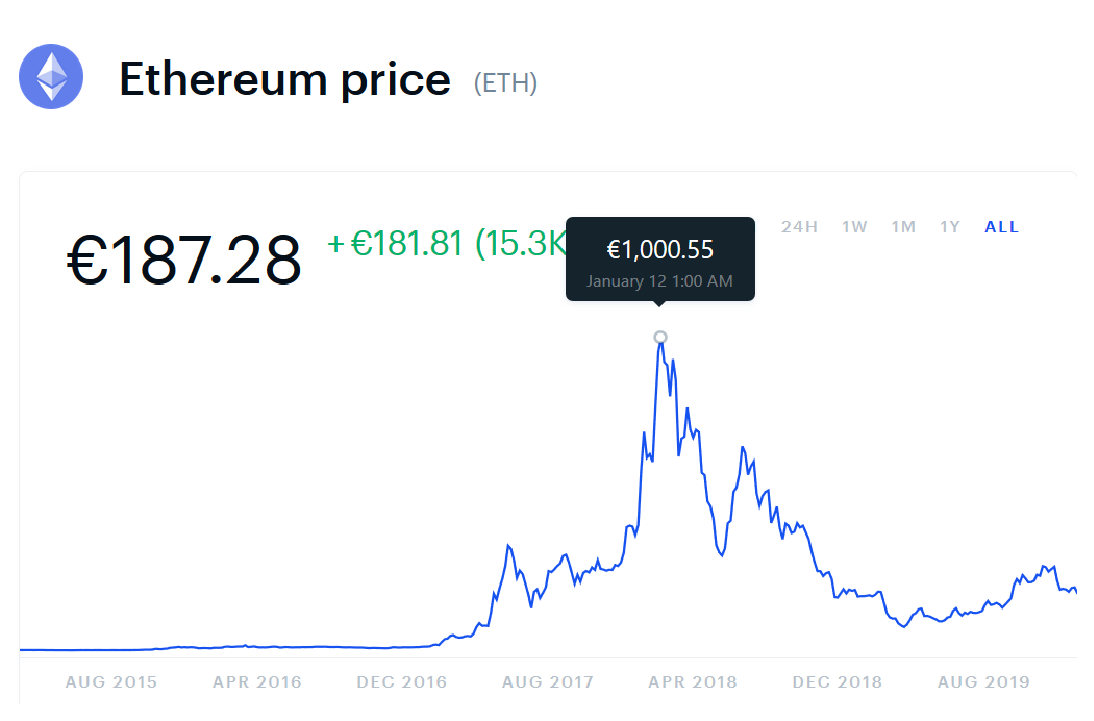
\includegraphics[keepaspectratio, width=0.481125\textwidth]{images/ethcurrentprice-sourcecoinbase.eps}
%  \caption{Figura 3. Variación cotización ETH (11/08/2019)}
%\end{figure}
\\
Figura 3. Variación cotización ETH (11/08/2019). Fuente: [Coinbase 19]
\\
\end{center}
(Por completar)
\section{Líneas futuras}\label{sec:future}
Como líneas futuras y complemento a este trabajo, con más tiempo, se plantea:
\subsection{Añadir forma de pago DAI} \label{ch:dai}
DAI es una criptomoneda estable (\textit{stablecoin}) que funciona con ETH y que intenta mantener un valor de 1\$. A diferencia de los billetes de banco centralizados, DAI no está respaldado por dólares estadounidenses en una cuenta bancaria. En cambio, está respaldado por garantías en la plataforma Maker [MakerDAO 19].
\subsection{Usar Raspberry Pi 4 Modelo B} \label{ch:rpi4modelb}
Anunciado en Junio de 2019 y a la venta. Es un hardware que ofrece mejores prestaciones. Por ejemplo, el procesador es un Broadcom BCM2711. Un ARM Cortex-A72 de cuatro núcleos y a 1,5 GHz. Hasta tres veces más eficiente (\textit{benchmark}) que el modelo anterior (Raspberry Pi 3 Modelo B+). También da la posibilidad de elegir entre 1, 2 y 4 GB de RAM.
\subsection{Usar Docker Swarm} \label{ch:dockerswarm}
Se podría presentar una aplicación descentralizada basada en microservicios. Por ejemplo en microservicios, un contenedor Docker (como en la sección 4) podría verse como un servicio. Entre las ventajas que aporta microservicios estarían:
\begin{itemize}
 \item Pequeños
 \item Independientes
 \item Despliegue sencillo
 \item Reutilizables
 \item Externalización
 \item Escalabilidad
 \newline
\end{itemize}
Para ello, Docker ofrece un orquestador (de código abierto) llamado Docker Swarm (véase figura 4). Un nodo \textit{worker} sería nuestra Raspberry Pi y un nodo \textit{manager} sería un centro de control.
\begin{center}
%\begin{figure}[h]
%  \centering
  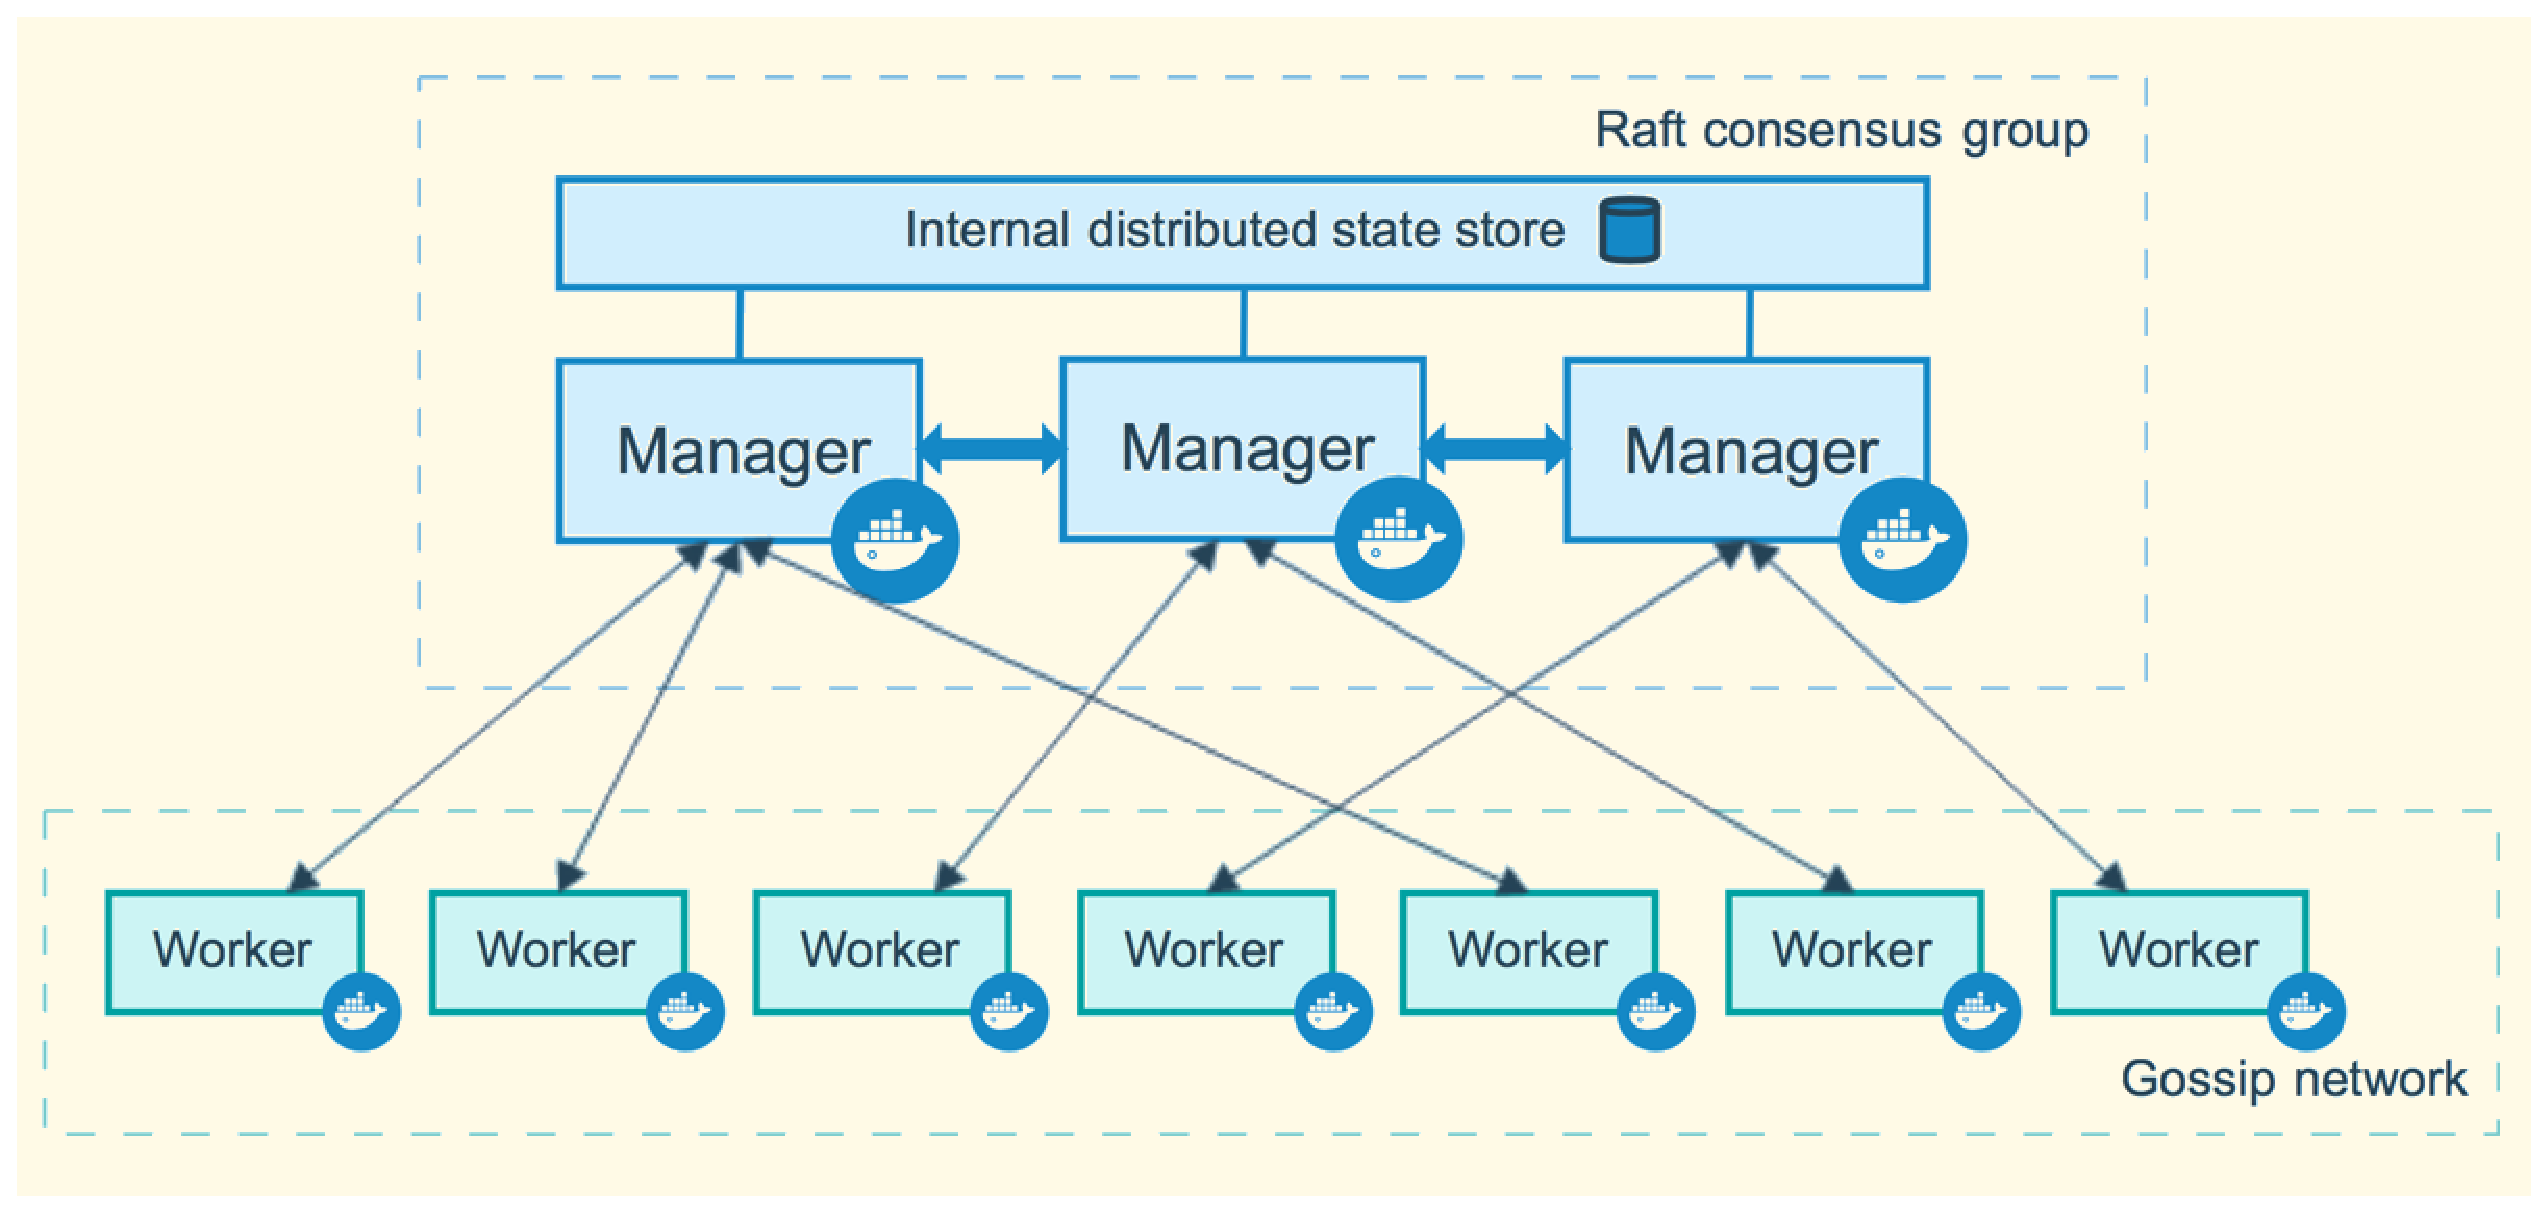
\includegraphics[keepaspectratio, width=0.481125\textwidth]{images/swarm-diagram-sourcedocker.eps}
%  \caption{Figura 3. Variación cotización ETH (11/08/2019)}
%\end{figure}
\\
Figura 4. Diagrama Docker Swarm. Fuente: [Docker 19]
\\
\end{center}
\section{Repositorio}\label{sec:repository}
El código fuente generado en el proyecto está publicado en un repositorio público de GitHub bajo licencia MIT.
\newline\newline
\url{https://github.com/ethereum-internet-access}
\newline
\begin{thebibliography}{9}
\bibitem{Coinbase19} Coinbase. Intercambio de moneda digital \href{https://www.coinbase.com/price/ethereum}{https://www.coinbase.com/price/ethereum}
\bibitem{ConsenSys19} Ethereum Smart Contract Best Practices. Security tools. ConsenSys. 12 Agosto 2019.
\bibitem{Docker19} Docker Documentation. How nodes work. 6 Septiembre 2019.  \href{https://docs.docker.com/engine/swarm/how-swarm-mode-works/nodes/}{https://docs.docker.com/engine/swarm/how-swarm-mode-works/nodes/}
\bibitem{ETHBerlinZwei19} Hackathon ETH Berlín Zwei. Twitter. 6 Septiembre 2019. \href{https://twitter.com/ETHBerlin}{https://twitter.com/ETHBerlin}
\bibitem{Hegedus18} P. Hegedus. "Towards Analyzing the Complexity Landscape of Solidity Based Ethereum Smart Contracts". 2018 IEEE/ACM 1st International Workshop on Emerging Trends in Software Engineering for Blockchain (WETSEB). 27 Mayo-3 Junio 2018. \href{https://ieeexplore.ieee.org/document/8445056}{https://ieeexplore.ieee.org/document/8445056}
\bibitem{MakerDAO19} MakerDAO. Stability for the blockchain.  \href{https://makerdao.com/en/dai}{https://makerdao.com/en/dai}
\bibitem{Munoz18} J. L. Muñoz. "Docker Containers". Apuntes de las clases magistrales. Máster en Tecnologías Blockchain. 1, Edición. UPC School. 29 Noviembre 2018.
\bibitem{Nakamoto08} S. Nakamoto. "Bitcoin: A Peer-to-Peer Electronic Cash System". 31 Octubre 2008.  \href{https://bitcoin.org/bitcoin.pdf}{https://bitcoin.org/bitcoin.pdf}
\bibitem{RaspberryPi19} Raspberry Pi 3 Modelo B - Placa Base (1,2 GHz Quad-Core Arm Cortex-A53, 1 GB RAM, USB 2.0). Amazon. 11 Agosto 2019.
\bibitem{RaspberryPiBuy19} Raspberry Pi FAQs. BUYING AND SHIPPING. Where can I buy a Raspberry Pi?. Página Web oficial. 11 Agosto 2019.  \href{https://www.raspberrypi.org/help/faqs/#buyingWhere}{https://www.raspberrypi.org/help/faqs/\#buyingWhere}
\bibitem{Stallings04} W. Stallings. "Comunicaciones y redes de computadores". 1 Septiembre 2004. Páginas 904. Pearson Prentice Hall. ISBN-13: 978-8420541105.
\end{thebibliography}
\clearpage

\end{multicols}


\end{document}
